% Options for packages loaded elsewhere
\PassOptionsToPackage{unicode}{hyperref}
\PassOptionsToPackage{hyphens}{url}
\PassOptionsToPackage{dvipsnames,svgnames,x11names}{xcolor}
%
\documentclass[
  letterpaper,
  DIV=11,
  numbers=noendperiod]{scrartcl}

\usepackage{amsmath,amssymb}
\usepackage{iftex}
\ifPDFTeX
  \usepackage[T1]{fontenc}
  \usepackage[utf8]{inputenc}
  \usepackage{textcomp} % provide euro and other symbols
\else % if luatex or xetex
  \usepackage{unicode-math}
  \defaultfontfeatures{Scale=MatchLowercase}
  \defaultfontfeatures[\rmfamily]{Ligatures=TeX,Scale=1}
\fi
\usepackage{lmodern}
\ifPDFTeX\else  
    % xetex/luatex font selection
\fi
% Use upquote if available, for straight quotes in verbatim environments
\IfFileExists{upquote.sty}{\usepackage{upquote}}{}
\IfFileExists{microtype.sty}{% use microtype if available
  \usepackage[]{microtype}
  \UseMicrotypeSet[protrusion]{basicmath} % disable protrusion for tt fonts
}{}
\makeatletter
\@ifundefined{KOMAClassName}{% if non-KOMA class
  \IfFileExists{parskip.sty}{%
    \usepackage{parskip}
  }{% else
    \setlength{\parindent}{0pt}
    \setlength{\parskip}{6pt plus 2pt minus 1pt}}
}{% if KOMA class
  \KOMAoptions{parskip=half}}
\makeatother
\usepackage{xcolor}
\setlength{\emergencystretch}{3em} % prevent overfull lines
\setcounter{secnumdepth}{-\maxdimen} % remove section numbering
% Make \paragraph and \subparagraph free-standing
\ifx\paragraph\undefined\else
  \let\oldparagraph\paragraph
  \renewcommand{\paragraph}[1]{\oldparagraph{#1}\mbox{}}
\fi
\ifx\subparagraph\undefined\else
  \let\oldsubparagraph\subparagraph
  \renewcommand{\subparagraph}[1]{\oldsubparagraph{#1}\mbox{}}
\fi


\providecommand{\tightlist}{%
  \setlength{\itemsep}{0pt}\setlength{\parskip}{0pt}}\usepackage{longtable,booktabs,array}
\usepackage{calc} % for calculating minipage widths
% Correct order of tables after \paragraph or \subparagraph
\usepackage{etoolbox}
\makeatletter
\patchcmd\longtable{\par}{\if@noskipsec\mbox{}\fi\par}{}{}
\makeatother
% Allow footnotes in longtable head/foot
\IfFileExists{footnotehyper.sty}{\usepackage{footnotehyper}}{\usepackage{footnote}}
\makesavenoteenv{longtable}
\usepackage{graphicx}
\makeatletter
\def\maxwidth{\ifdim\Gin@nat@width>\linewidth\linewidth\else\Gin@nat@width\fi}
\def\maxheight{\ifdim\Gin@nat@height>\textheight\textheight\else\Gin@nat@height\fi}
\makeatother
% Scale images if necessary, so that they will not overflow the page
% margins by default, and it is still possible to overwrite the defaults
% using explicit options in \includegraphics[width, height, ...]{}
\setkeys{Gin}{width=\maxwidth,height=\maxheight,keepaspectratio}
% Set default figure placement to htbp
\makeatletter
\def\fps@figure{htbp}
\makeatother

\KOMAoption{captions}{tableheading}
\makeatletter
\@ifpackageloaded{caption}{}{\usepackage{caption}}
\AtBeginDocument{%
\ifdefined\contentsname
  \renewcommand*\contentsname{Table of contents}
\else
  \newcommand\contentsname{Table of contents}
\fi
\ifdefined\listfigurename
  \renewcommand*\listfigurename{List of Figures}
\else
  \newcommand\listfigurename{List of Figures}
\fi
\ifdefined\listtablename
  \renewcommand*\listtablename{List of Tables}
\else
  \newcommand\listtablename{List of Tables}
\fi
\ifdefined\figurename
  \renewcommand*\figurename{Figure}
\else
  \newcommand\figurename{Figure}
\fi
\ifdefined\tablename
  \renewcommand*\tablename{Table}
\else
  \newcommand\tablename{Table}
\fi
}
\@ifpackageloaded{float}{}{\usepackage{float}}
\floatstyle{ruled}
\@ifundefined{c@chapter}{\newfloat{codelisting}{h}{lop}}{\newfloat{codelisting}{h}{lop}[chapter]}
\floatname{codelisting}{Listing}
\newcommand*\listoflistings{\listof{codelisting}{List of Listings}}
\makeatother
\makeatletter
\makeatother
\makeatletter
\@ifpackageloaded{caption}{}{\usepackage{caption}}
\@ifpackageloaded{subcaption}{}{\usepackage{subcaption}}
\makeatother
\ifLuaTeX
  \usepackage{selnolig}  % disable illegal ligatures
\fi
\usepackage{bookmark}

\IfFileExists{xurl.sty}{\usepackage{xurl}}{} % add URL line breaks if available
\urlstyle{same} % disable monospaced font for URLs
\hypersetup{
  pdftitle={Bericht Steinschlagrisiko},
  pdfauthor={Livio Prosdocimo, Roberto Lorusso, Linus Ackermann},
  colorlinks=true,
  linkcolor={blue},
  filecolor={Maroon},
  citecolor={Blue},
  urlcolor={Blue},
  pdfcreator={LaTeX via pandoc}}

\title{Bericht Steinschlagrisiko}
\usepackage{etoolbox}
\makeatletter
\providecommand{\subtitle}[1]{% add subtitle to \maketitle
  \apptocmd{\@title}{\par {\large #1 \par}}{}{}
}
\makeatother
\subtitle{Challenge CWM1}
\author{Livio Prosdocimo, Roberto Lorusso, Linus Ackermann}
\date{10.06.2024}

\begin{document}
\maketitle

\renewcommand*\contentsname{Inhaltsverzeichnis}
{
\hypersetup{linkcolor=}
\setcounter{tocdepth}{3}
\tableofcontents
}
\newpage

\section{Problem}\label{problem}

Die Kantonsstrasse nach Schiers GB ist von Steinschlägen betroffen. Um
die Sicherheit der Verkehrsteilnehmer zu gewährleisten, wurde im Auftrag
des Kantonsingenieurs diese Risikoanalyse erstellt.

An zwei Stellen des Hangs fallen täglich Steine herunter. Bevor diese
die Strasse erreichen, werden sie von Fangnetzen aufgehalten. Diese
Netze können eine bestimmte Menge an Energie von herabfallenden Steinen
aufnehmen. Wenn jedoch Steine in den Netzen liegen, verringert sich ihre
Haltekraft. Die Netze werden täglich geräumt. Durch die Abnutzung der
Netze hat sich die Stabilität beeinträchtigt und das Risiko erhöht.

Es muss entschieden werden, ob eine Strassensperrung unvermeidlich ist.
Diese Analyse soll die Basis für die Entscheidung des Kantonsingenieurs
bilden.

\section{Wahrscheinlichkeitsmodellierung}\label{wahrscheinlichkeitsmodellierung}

Die Bestimmung einer Strassensperrung besteht in der Ermittlung der
modellierten Wahrscheinlichkeit für einen Todesfall infolge eines
Steinschlags. Dabei ist eine Berücksichtigung diverser Variablen
erforderlich, welche einen Einfluss auf einen tatsächlichen Todesfall
ausüben. Die Zusammensetzung dieser Variablen determiniert die
Gesamtwahrscheinlichkeit für einen Todesfall, welche eine Jährliche
Wahrscheinlichkeit von 0.002 nicht überschreiten darf, um das Risiko
auszuschliessen.

\newpage

\subsection{Zufallsvariablen}\label{zufallsvariablen}

Im ersten Schritt muss ein Todesfall simuliert und die Schritte bis zu
diesem Ereignis analysiert werden, um die relevanten Variablen zu
identifizieren.

Ein Steinschlag mit einer so grossen Energie, dass die Netze reissen,
ist erforderlich, damit eine Verkehrsperson auf dieser Strasse ums Leben
kommen könnte. Ausserdem muss sich während dieses durchbrechenden
Steinschlags ein Fahrer in der Todeszone befinden. Die Todeszone
bezeichnet den Bereich, in dem eine Reaktion nicht mehr möglich ist und
ein Zusammenprall unausweichlich ist.

Zunächst sind die Umstände zu eruieren, unter denen ein Steinschlag ein
Netz durchbrechen kann. Zu diesem Zweck wurden durch Expertisen folgende
Kriterien anhand gesammelten Daten definiert.

\begin{itemize}
\tightlist
\item
  Ein Steinschlag bricht durch, wenn die Energie 1200 kNm übersteigt.
\item
  Ebenso reissen die Netze, wenn das Gewicht der bereits im Netz
  befindlichen Steine, also der vorherigen Steinschlägen, über 2000 kg
  beträgt. In diesem Fall erfolgt ein Reissen der Netze bereits bei
  einem Steinschlag von 600 kNm.
\item
  Die Entfernung der Steine im Netz erfolgt durch ein vor Ort
  stationiertes Team, welches spätestens alle 24 Stunden tätig wird.
\end{itemize}

Somit müssen folgende Eigenschaften eines Steinschlags berücksichtigt
werden, um die Wahrscheinlichkeit eines Durchbruchs zu definieren:

\begin{itemize}
\item
  Geschwindigkeit und Masse der Steinschläge: Diese sind erforderlich,
  um die Energie eines Steinschlags zu berechnen.
\item
  Die zeitlichen Abstände zwischen den Steinschlägen und deren Masse:
  Diese Informationen sind notwendig, um herauszufinden, wie viele
  Steine sich noch im Netz befinden könnten und welche Masse sie haben.
\end{itemize}

Um diese beiden Aspekte zu ermitteln, benötigen wir Daten über die
Masse, Geschwindigkeit und zeitlichen Abständen der Steine. Experten und
Geologen haben diese Daten in den letzten Monaten bei den vorkommenden
Steinschlägen gesammelt und für die Modellierung zur Verfügung gestellt.
Diese Daten bilden die Grundlage für diese Analyse.

In den folgenden Abschnitten wird die Berechnung bis zum Durchbrechen
eines Fangnetzes durch einen Steinschlag behandelt. Die Todeszone wird
am Schluss der Analyse bei der Gesamtkalkulation berücksichtigt.

\subsection{Verteilungen}\label{verteilungen}

Da Steinschläge über einen Zeitraum von drei Monaten aufgrund der
begrenzten Anzahl an Ereignissen keine verlässlichen Aussagen über die
aktuelle Gefahr ermöglichen, müssen Fälle nachgestellt werden und zwar
möglichst viele. Um eine solche Simulation korrekt durchzuführen, werden
die vorhandenen Daten der Steinschläge in die genannten Variablen Masse,
Geschwindigkeit und zeitliche Abstände unterteilt.

Dann können diese Daten anhand ihren Eigenschaften simuliert werden.
Davor wird aber jeder Variable eine Wahrscheinlichkeitsverteilung
zugeordnet. Durch die Zuordnung können Fälle repdorduziert werden,
welche die Eigenschaften der Daten anhand den gewählten theoretischen
Modellen widerspiegelen. Im nächsten Schritt werden den Variablen
Verteilungen zugeteilt. Da zwei stellen an der Strasse von Steinschläge
betroffen sind, müssen diese getrennt betrachtet werden, Beide Hänge
haben ihre eigenen Eigenschaften bezüglich Masse, Geschwindigkeit und
den Zeitlichen Unterscherschiede.

\subsubsection{Wahl der Verteilungen}\label{wahl-der-verteilungen}

Mit dem fitdistr-Package können die verschiedenen Verteilungen auf die
Daten angewendet werden.

Alle verwendeten Verteilungen durchlaufen dann einen Prozess, in dem die
am besten geeignete Verteilung ermittelt wird. Der Prozess ist folgend
durchgeführt worden:

\begin{itemize}
\item
  Zunächst wird ein Histogramm der Daten mit den Verteilungen als Linien
  betrachtet. Die Verteilungen, welche den Balken besser folgen sind
  eher geeignet.
\item
  In einem Cullen-Frey-Diagramm, werden die Datenpunkte zusammen mit den
  Verteilungen verglichen. Die Verteilungen, die am nächsten an den
  Beobachtungspunkten liegen, sind tendenziell besser geignet.
\item
  Mit der Funktion UnivariateML können verschiedene Verteilungen bereits
  im Vorhinein getestet werden, um herauszufinden, welche am besten zu
  den Daten passt. Diese Funktion vergleicht die Kompatibilität der
  Daten mit verschiedenen Verteilungen und bietet somit eine
  Möglichkeit, eine mögliche Passform für die vorliegenden Daten zu
  ermitteln. Diese Funktion unterstützt die Auswahl von den
  verschiedenen Verteilungen.
\end{itemize}

Diese drei Schritte allein erlauben noch keine endgültige Entscheidung
darüber, welche Verteilung am besten geeignet ist. Sie dienen jedoch
dazu, die Auswahl der möglichen Verteilungen einzuschränken und eine
Orientierung zu geben, mit welchen Daten gearbeitet wird.

\begin{itemize}
\tightlist
\item
  Nachdem nun einige Verteilungen ausgeschlossen werden konnten, kann
  man sich den möglichen Verteilungen zuwenden. Man betrachtet die
  Verteilungen anhand von CDF-, QQ- und PP-Plots. Die Punkte in den
  Plots stellen die vorhandenen Daten auf der Y-Achse dar, im Vergleich
  zu den theoretischen Werten, welche die Verteilung erzeugt, auf der
  X-Achse. Danach kann eine endgültige Entscheidung getroffen werden.
\end{itemize}

In Fällen, in denen die Verteilungen ähnlich sind und eine Entscheidung
schwierig ist, sollte Folgendes berücksichtigt werden.

-Grössere Massen und grössere Geschwindigkeit bedeuten ein höheres
Risiko, daher ist es wichtiger, die grössten Daten auf den QQ-, CDF- und
PP-Plots abzudecken, als kleinere Daten.

\begin{itemize}
\tightlist
\item
  Bei den Zeitlichen Abständen sind kleinere Daten wichtiger, da weniger
  Zeitintervalle mehrere Steinschläge bedeuten und somit eine grössere
  Gefahr darstellen. In diesem Fall ist es wichtiger, die kleineren
  Daten in den QQ-, CDF- und PP-Plots abzudecken, als die grossen.
\end{itemize}

Im nächsten Abschnitt befindet sich die Anwendung dieses Prozess auf
beide Hänge.

\subsubsection{Zone 1 Masse}\label{zone-1-masse}

Zunächst wird die Zone 1 hinsichtlich Masse untersucht. Beim
Ausschlussverfahren zeigt sich, dass nur die Weibull- und die
Lognormalverteilung in Frage kommen könnten. Der Vorschlag von
UnivariateML ist die Lognormalverteilung.

Vergleicht man die Masse am Zone 1 zwischen der Lognormalverteilung und
der Weibullverteilung, so würde die Lognormalverteilung insgesamt besser
die Daten abdecken, nur das letzte Quantil im QQ-Plot weicht deutlich
ab.

Bei der Weibullverteilung weichen die Punkte ebenfalls von der Linie ab,
aber insbesondere die letzten Quantile passen zu dieser Verteilung.

Trotz kleiner Abweichungen wird die Weibull-Verteilung zugewiesen.
Gemäss letztem Schritt im Prozess ist es wichtig, dass die grössten
Massen gedeckt sind.

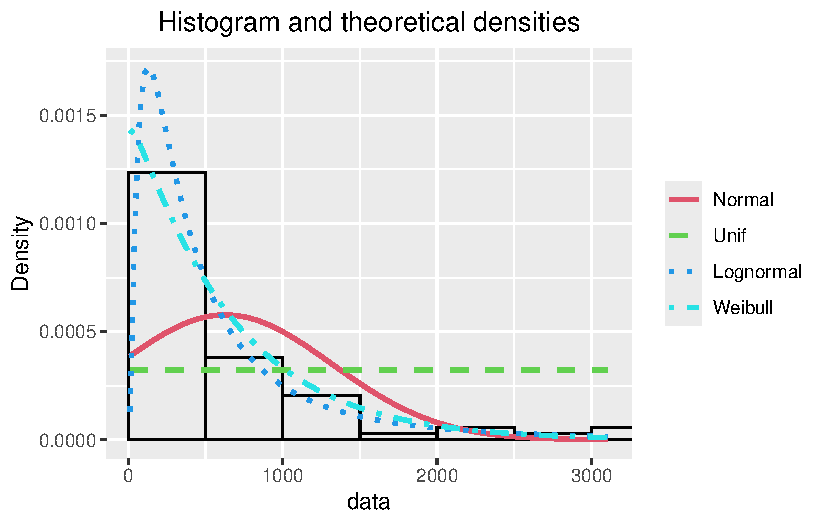
\includegraphics{steinschlag_bericht_files/figure-pdf/unnamed-chunk-4-1.pdf}

\subsubsection{Zone 1 Geschwindigkeit}\label{zone-1-geschwindigkeit}

Durch die erste Analyse filtert sich heraus, dass die Normal-, Weibull-,
Exponential-, Gamma-, und Lognormalverteilung passen könnten.

Der Vorschlag von UnivariateML ist die Normalverteilung.

Nach dem Abgleich der Plots ist klar, dass die Normalverteilung am
besten passt. Die Punkte verlaufen fast durchgehend entlang der Linie.
Besonders in den oberen Werten ist diese Verteilung am nächsten bei der
Linie. Daher wird die Normalverteilung zugewiesen.

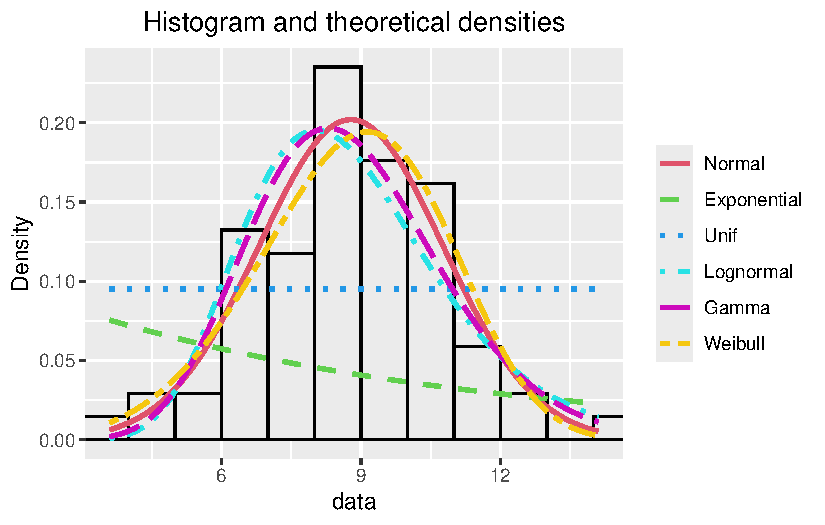
\includegraphics{steinschlag_bericht_files/figure-pdf/unnamed-chunk-6-1.pdf}

\subsubsection{Zone 1 Zeitabstände}\label{zone-1-zeitabstuxe4nde}

Die erste Analyse deutet in diesem Fall klar darauf hin, dass nur eine
Exponential- oder Normalverteilung passend sein könnten.

Der Vorschlag von UnivariateML ist die Exponentialverteilung.

Die Auswertung der Plots zeigt deutlich, dass die Exponentialverteilung
am besten passt. Die kleineren Werte werden bei der
Exponentialverteilung besser gedeckt. Die anderen Verteilungen weichen
fest von der Linie ab. Daher wird die Exponentialverteilung zugewiesen.

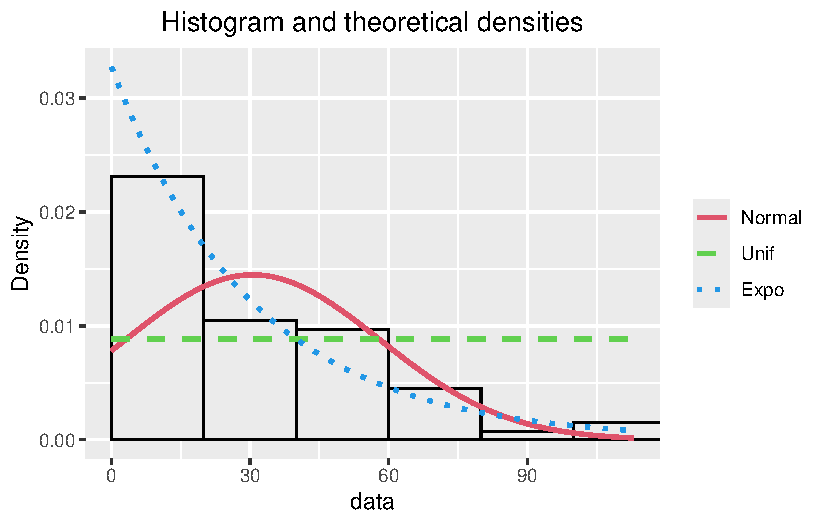
\includegraphics{steinschlag_bericht_files/figure-pdf/unnamed-chunk-8-1.pdf}

\subsubsection{Zone 2 Masse}\label{zone-2-masse}

Nach einer ersten Prüfung bleiben die Verteilungen Weibull, Gamma,
Exponential und Lognormal zur Auswahl.

Der Vorschlag von UnivariateML ist die Exponentialverteilung.

Nach Bewertung der Plots wird die Exponentialverteilung zugewiesen.
Gamma- und Weibullverteilungen sind zwar ähnlich wie die
Exponentialverteilung, decken aber die oberen Werte schlechter ab.
Lognormal liegt im Allgemeinen näher an der Linie, berücksichtigt aber
den höchsten Wert nicht.

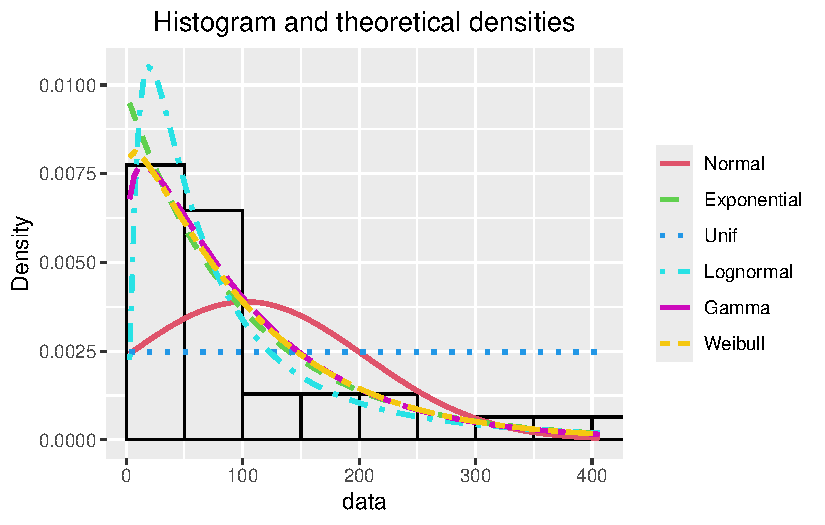
\includegraphics{steinschlag_bericht_files/figure-pdf/unnamed-chunk-11-1.pdf}

\subsubsection{Zone 2 Geschwindigkeit}\label{zone-2-geschwindigkeit}

Beim Ausschlusserfahren erkennt man, dass viele Verteilungen ausgewählt
werden könnten. Normal-, Lognormal-, Weibull- und Gammaverteilung stehen
zur Auswahl.

Der Vorschlag von UnivariateML ist die Weibullverteilung.

Die Auswertung zeigt, dass nur die Weibullverteilung die Daten
umfangreich decken kann. Daher wird diese Verteilung zugewiesen.

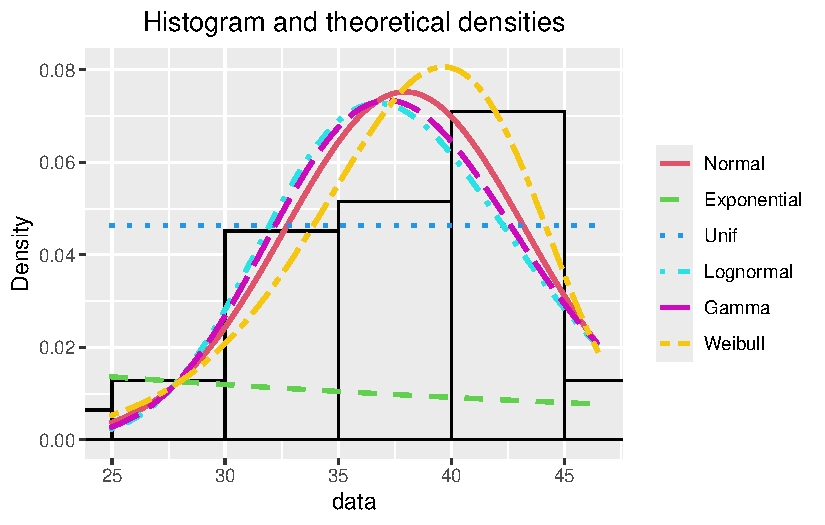
\includegraphics{steinschlag_bericht_files/figure-pdf/unnamed-chunk-13-1.pdf}

\subsubsection{Zone 2 Zeitabstände}\label{zone-2-zeitabstuxe4nde}

Nach der ersten Prüfung kann man die Auswahl auf Weibull-, Gamma-,
Exponential- und Lognormalverteilung reduzieren.

Der Vorschlag von UnivariateML ist die Gammaverteilung.

Beim Vergleich fällt schnell auf, dass Gamma- und Weibullverteilungen
die einzigen Modelle sind, welche in Frage kommen. Die korrekte
Verteilung in diesem Fall ist die Gammaverteilung, da diese sowohl der
Empfehlung von UnivariateML entspricht als auch die unteren Werte besser
abdeckt.

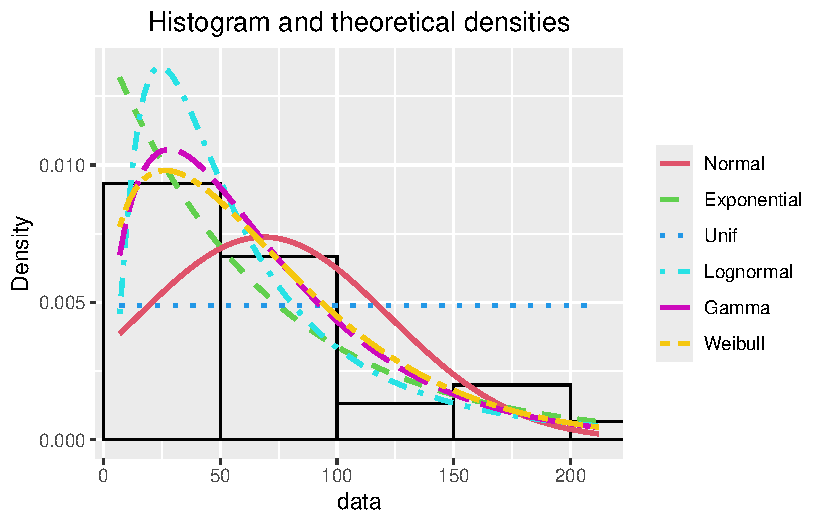
\includegraphics{steinschlag_bericht_files/figure-pdf/unnamed-chunk-15-1.pdf}

\newpage

\subsubsection{Gewählte Verteilungen}\label{gewuxe4hlte-verteilungen}

In der folgenden Tabelle ist ersichtlich, welche Verteilungsfunktionen
gewählt wurden. Die Parameter sind die ausgerechneten Werte, welche für
das Generieren anhand der Verteilungsfunktion benötigt werden.

\begin{longtable}[]{@{}
  >{\raggedright\arraybackslash}p{(\columnwidth - 8\tabcolsep) * \real{0.2000}}
  >{\raggedright\arraybackslash}p{(\columnwidth - 8\tabcolsep) * \real{0.2000}}
  >{\raggedright\arraybackslash}p{(\columnwidth - 8\tabcolsep) * \real{0.2000}}
  >{\raggedright\arraybackslash}p{(\columnwidth - 8\tabcolsep) * \real{0.2000}}
  >{\raggedright\arraybackslash}p{(\columnwidth - 8\tabcolsep) * \real{0.2000}}@{}}
\toprule\noalign{}
\begin{minipage}[b]{\linewidth}\raggedright
Zufallsvariable
\end{minipage} & \begin{minipage}[b]{\linewidth}\raggedright
Zone
\end{minipage} & \begin{minipage}[b]{\linewidth}\raggedright
Verteilung
\end{minipage} & \begin{minipage}[b]{\linewidth}\raggedright
Parameter 1
\end{minipage} & \begin{minipage}[b]{\linewidth}\raggedright
Parameter 2
\end{minipage} \\
\midrule\noalign{}
\endhead
\bottomrule\noalign{}
\endlastfoot
Masse & 1 & Weibul & 1.0258858 & 636.1013056 \\
Geschwindigkeit & 1 & Normal & 8.7882353 & 1.9745088 \\
Zeitabstand & 1 & Exponential & 0.0327308 & \\
Masse & 2 & Exponential & 0.0097607 & \\
Geschwindigkeit & 2 & Weibul & 8.7882353 & 1.9745088 \\
Zeitabstand & 2 & Gamma & 0.0327308 & \\
\end{longtable}

\section{Simulation}\label{simulation}

Nun sind den Zufallsvariablen Verteilungen zugeordnet. Der nächste
Schritt ist die Simulation.

\subsection{Generieren}\label{generieren}

Das Generieren der Zufallsveriablen wurde mit R umgesetzt. Dabei wurden
die Daten anhand der \hyperref[gewuxe4hlte-verteilungen]{gewählten
Verteilungen} zufällig generiert. Insgesamt wurde für jede Zone
\textbf{10000000} Steinschläge generiert.

Die Kinetische Energie wird anhand der Geschwindigkeit und Masse eines
Steinschlags, mittels der Physikalischen Formel berechnet und in Kilo
Newton Meter umgewandelt.

\[
E_{\text{kin}} = \frac{1}{2} \times m \times v^{2}
\]\newline

\newpage

\subsection{Wahrscheinlichkeitsberechnung}\label{wahrscheinlichkeitsberechnung}

Durch die Simulation von Steinschlägen ist es nun möglich, die
Wahrscheinlichkeit eines Todesfalls zu berechnen. Mit den folgenden
Angaben ist es möglich, die Wahrscheinlichkeit, dass das Sicherheitsnetz
reisst je Steinschlag, auszurechnen. Dafür verwenden wir folgende
Formel. Dass bei einem Steinschlag die Sicherheitsnetze reissen, müsste
die kinetische Energie höher sein als 1200 kNm oder 600 kNm und die
Masse im Sicherheitsnetz grösser oder gleich 2000 kg sein. Das
Sicherheitsnetz wird alle 24 Stunden geleert. Um in der Simulation die
Masse im Netz bei einem Steinschlag zu berechnen, werden rekursiv alle
vergangenen Steinschläge, welche in den letzten 24 Stunden stattgefunden
haben, durchlaufen und die Masse aufsummiert. Dadurch wird es
ermöglicht, alle Steinschläge herauszufiltern, welche eine kinetische
Energie von mindestens 1200 kNm haben oder mindestens 600 kNm und im
Sicherheitsnetz eine Gesamtmasse von 2000 kg liegen.

Mit diesen Angaben ist es möglich, die Wahrscheinlichkeit, dass das
Sicherheitsnetz reisst, auszurechnen. Dafür verwenden wir folgende
Formel.

\[
P_{\text{Netz reisst}} = \frac{\text{Anzahl Netz Versagen}}{\text{Anzahl Steinschläge}} 
\]

Das ein Steinschlag in einem Todesfall endet muss zusätzlich ein Auto
sich in der Todeszone befinden. Um die Wahrscheinlichkeit dafür zu
berechnen wird die Zeit benötigt, welches ein Auto benötigt um für einen
Möglichen Steinschlag zu bremsen. Dies lässt sich aus dem Bremsweg, was
sich bei einer
\href{https://www.adac.de/verkehr/rund-um-den-fuehrerschein/erwerb/anhalteweg-berechnen/}{Gefahrenbesmung
bei 18m} liegt, bei einer Geschwindigkeit von 60 km/h und der
Geschwindigkeit, wie folgt berechnen.

\[
t = \frac{2s}{v} \Rightarrow \frac{2\times18m}{16.\overline{6}m/s} \approx 2.16s 
\]

Dazu wird noch die
\href{https://www.adac.de/verkehr/rund-um-den-fuehrerschein/erwerb/reaktionsweg-berechnen/}{Vorbremszeit
von 1.2 Sekunde} addiert, welche ein Mensch braucht um auf die Bremse zu
drücken. Damit kommt man auf \emph{3.36 Sekunden}, welche ein Auto in
der Gefahrenzone ist. Durch diesen Wert können wir die
Wahrscheinlichkeit berechnen, dass ein Auto zu einem beliebigen
Zeitpunkt in der Gefahrenzone ist.

\[
P_{\text{Auto anwesend}} = \frac{3.36 \times \text{Anazhl Autos Pro Tag}}{\text{Anzahl Sekunden Pro Tag}} \Rightarrow \frac{3.36 \times 600}{86400} = \frac{7}{300}
\]

Mit der Wahrscheinlichkeit, dass das Sicherheitsnetz reisst, ein Auto
anwesend ist und der durchschnittlichen Steinschläge pro Jahr, lässt
sich die Wahrscheinlichkeit eines tödlichen Unfalls in einer Zone für
ein Jahr berechnen.

\[
P_{\text{Tödlicher Unfall pro Jahr}} = P_{\text{Auto anwesend}} \times P_{\text{Netz reisst}} \times \text{ Durchschnittliche Steinschläge pro Jahr}
\]

\newpage

\section{Ergebniss}\label{ergebniss}

\subsection{Zone 1}\label{zone-1}

Die Simulation von 10000000 Steinschlägen in der Zone 1 ergab, dass 0
Steinschläge durch das Sicherheitsnetz gingen. Dabei wurden
34866.1255739 Jahre an Steinschlägen simuliert. Wobei jährlich im
Schnitt 286.8113344 Steinschläge herunterkommen. Daraus resultiert, eine
Wahrscheinlichkeit von \textbf{0} pro Jahr, dass ein Unfall passiert.

\subsection{Zone 2}\label{zone-2}

Die Simulation von 10000000 Steinschlägen in der Zone 2 ergab, dass 27
Steinschläge durch das Sicherheitsnetz gingen. Dabei wurden
78229.3429922 Jahre an Steinschlägen simuliert. Wobei jährlich im
Schnitt 127.8292725 Steinschläge herunterkommen. Daraus resultiert, eine
Wahrscheinlichkeit von \textbf{0.0000081} pro Jahr, dass ein Unfall
passiert.

\subsection{Gesammt}\label{gesammt}

Das Verbinden der Wahrscheinlichkeiten, dass ein Unfall in Folge
Steinschläge auf der Kantonsstrasse. Wird mit der folgenden Formel
berechnet. \[
P_{\text{Todesfall}}(P_{\text{Todesfall Zone 1}} \cup P_{\text{Todesfall Zone 2}})
\] Daraus resultiert eine Wahrscheinlichkeit eines Unfalls in Folge
eines Steinschlages von \textbf{0.0000081}

\section{Empfehlung}\label{empfehlung}

Auf Basis der durchgeführten Simulation und Analyse der Daten, welche
eine geringere jährliche Wahrscheinlichkeit als die Obergrenze von 0.002
ergeben hat. Empfehlen wir dem Kantonsingenieur, die Kantonsstrasse
unterhalb Schiers (GR) nicht zu schliessen.



\end{document}
